\chapter{Implemenations and Evaluations}

This chapter presents details of the implementations, experiments and evaluations for the proposed models in previous chapter. Section \ref{sec:chap4_implementation} describes the architecture of training system written in Torch framework which was used to train all the models. Before going onto detailed experiments and evaluations, section \ref{sec:chap4_metric} provides explanation for the metrics used to evaluate models' performances includeng BLUE, METEOR and CIDEr scores. Subsequently, section \ref{sec:chap4_experiment} presents all the experiments along with evaluation and assessment for each of them.

%% -------------------------------------
%% SECTION 1:
%%   Implementations
%% -------------------------------------
\section{Implementations}
\label{sec:chap4_implementation}


\subsection{Training System Architecture}

\subsection{Training and Monitoring}
Training a deep neural network can be very hard and time-consuming. During the course of training of all models and experiments presented in this thesis, I have followed several guidelines \cite{bottou-tricks-2012} on tips and tricks to effectively train deep neural networks.
	
	\subsubsection{Choosing a right learning rate}
	As shown in \cite{Murata98astatistical}, the mathematics of stochastic gradient descent do not depend on the size of training set. Therefore, the best way to determine the correct learning rates is to perform experiments on a small but representative traing set. When the model performs well on training cost with the sample training set with some learning rate $\gamma_t$, we can apply that learning rate to train our model on real training set.

	For this purpose, I set up a small experiment on subset of MSCOCO dataset (see \ref{sec:dataset_mscoco} for details). The subset COCO-1k consists of images randomly from MSCOCO training set. There are in total $1,200$ images in COCO-1k; $1,000$ of them are in training set and the rest are reserved in the validation set. I trained a model with 16-layer VGGNet as CNN; optimization method is SGD; the LSTM has 512 hidden units and with batch size equals to 5.

	\subsubsection{Monitoring the training process}
	\label{sec:monitoring}

%% -------------------------------------
%% SECTION 3:
%%   Experimental Environment
%% -------------------------------------
\section{Experimental Environment}
\label{sec:chap4_environment}

\subsection{Hardware configurations}
\label{sec:hardware}
All models are trained with the hardware configurations as shown in table \ref{tab:hardware_configuration}:

\begin{table}
	\centering
	\caption{Hardware configuration for training all models}	
	\label{tab:hardware_configuration}
	\begin{tabularx}{0.65\textwidth}{ll}
		\toprule
		CPU & 2 x Intel(R) Xeon(R) E5-2620v3 \\
			& (6 cores, 15MB cache, 2.40GHz) \\
		\midrule
		Memory & 4 x 32 GB ECC Registered \\
		\midrule 
		GPU & 2 x nVidia Tesla K80 [GK210B], \\
			& each with $2,496$ CUDA cores, \\
			& $12$GB VRAM, 240 GB/s memory bandwidth \\
		\midrule
		Storage & 8 x 6TB SATA 7200RPM Enterprise \\
		\bottomrule
	\end{tabularx}
\end{table}

\subsection{Datasets}
\subsubsection{Flickr8k}
Flickr8K was first proposed by \cite{Hodosh:2013:FID:2566972.2566993} as a benchmark collection for sentence-based image description and search. The dataset consists of $8,000$ images accompanied with five different description sentences which provide clear description of salient entities and events. \textit{TODO: re-paraphrase}
\subsubsection{Flickr30k}
As introduced in \cite{DBLP:journals/tacl/YoungLHH14}, Flickr30k is an extension of Flickr8k. The dataset is comprised of $158,915$ crowd-sourced captions describing $31,783$ images. Except for images that overlapped in Flickr8k, the new images and captions in this dataset focus on people involved in everyday activities and events.

Several examples of images and captions in Flickr8K and Flickr30k are shown in figure \ref{fig:flickr-examples}.

\begin{figure}
	\centering
	\label{fig:flickr-examples}
	\begin{tabular}{l l}
		\toprule
		\multirow{5}{*}{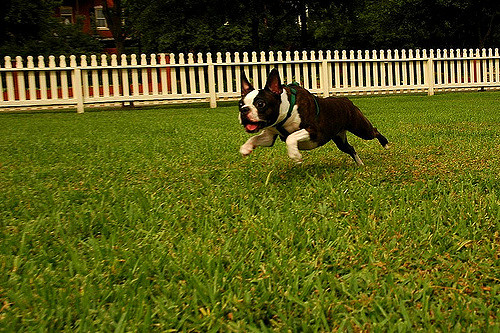
\includegraphics[width=0.25\linewidth]{Chapters/Fig/black_dog_running_fence.jpg}} & \parbox{11cm}{\small{A black and white dog is running in a grassy garden surrounded by a white fence}} \\
		& \small{A black and white dog is running through the grass} \\
		& \small{A Boston terrier is running in the grass} \\
		& \small{A Boston Terrier is running on lush green grass in front of a white fence} \\
		& \small{A dog runs on the green grass near a wooden fence} \\
		\midrule
		\begin{minipage}{0.25\linewidth}
			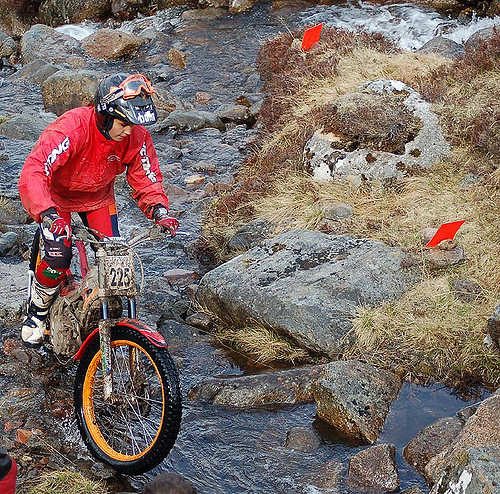
\includegraphics[width=\linewidth]{Chapters/Fig/men_red_helmet_riding_bike_rocks.jpg}
		\end{minipage}
		&
		\begin{minipage}{0.75\linewidth}
			\parbox{11cm}{\small{A boy in a black helmet and red long sleeve shirt rides his motorbike over a rocky stream}} \\
			\small{A man on a motorcycle steers through swampy terrain} \\
			\small{A man rides his bike over rocks and a creek.} \\
			\small{A motocross bike is being ridden between markers in a running stream.} \\
			\small{A person is dirt biking over rocks and water.}
		\end{minipage}\\
		\midrule
		\begin{minipage}{0.25\linewidth}
		IMAGE 335110163
			% \includegraphics[width=\linewidth]{Chapters/Fig/woman_photograph.png}
		\end{minipage}
		&
		\begin{minipage}{0.75\linewidth}
			\parbox{11cm}{\small{A woman with dark hair and a white shirt is taking a picture of an object at close range }} \\
			\parbox{11cm}{\small{A photographer taking a closeup photo of a glass perfume jar }} \\
			\parbox{11cm}{\small{A woman taking picture of her pet in her home }} \\
			\parbox{11cm}{\small{A woman taking a photo of an object on a bed }} \\
			\parbox{11cm}{\small{The lady is taking a closeup picture }} \\
		\end{minipage}\\
		\begin{minipage}{0.25\linewidth}
		IMAGE 908636680
			% \includegraphics[width=\linewidth]{Chapters/Fig/woman_photograph.png}
		\end{minipage}
		&
		\begin{minipage}{0.75\linewidth}
			\parbox{11cm}{\small{A group of eight campers sit around a fire pit trying to roast marshmallows on their sticks}} \\s
			\parbox{11cm}{\small{A group of men and women surrounding a bonfire while having conversation }} \\
			\parbox{11cm}{\small{Several people having fun and toasting marshmallows around a campfire }} \\
			\parbox{11cm}{\small{A group of people are outside , roasting marshmallows in a fire }} \\
			\parbox{11cm}{\small{Seven adults sit around a fire pit having a conversation }} \\
		\end{minipage}\\
		\bottomrule
	\end{tabular}
	\caption{Images with 5 crowd-sourced captions in Flickr8k and Flickr30k}
\end{figure}

\subsubsection{MSCOCO}
\label{sec:dataset_mscoco}

MSCOCO \cite{DBLP:journals/corr/LinMBHPRDZ14} (Microsoft Common Objects in Context) is a large-scale dataset that addresses three core research problems in scene understanding: detecting non-iconic views of objects, contextual reasoning between objects and the precise 2D localization of objects. It has been considered as the start-of-the-art dataset for numerous computer vision tasks (e.g., image classification, object detection, object segmentation, scene labelling, etc.). The dataset has approximately $328,000$ images of complex everyday scenes containing common objects in their natural context. Like in aforementioned Flickr8k \& Flickr30k datasets, each images in MSCOCO is also associated with five caption sentences that describe the content of such image.

The statistics of the datasets are summarized in table \ref{tab:dataset-statistics}
\begin{table}
	\centering
	\label{tab:dataset-statistics}
	\begin{tabular}{lccc}
		\toprule
		\multirow{2}{*}{Dataset name} & \multicolumn{3}{c}{size} \\ \cline{2-4}
		& train & validation & test \\ \midrule
		Flickr8k & 6000 & 1000 & 1000 \\
		Flickr30K & 28000 & 1000 & 1000 \\
		MSCOCO & 82783 & 40504 & 40775 \\
		\bottomrule
	\end{tabular}
	\caption{Dataset statistics}
\end{table}


%% -------------------------------------
%% SECTION 4:
%%   Experiments
%% -------------------------------------
\section{Experiments and Evaluations}
\label{sec:chap4_experiment}

This section gives the details of all experiments that I have conducted to explore and evaluate different models as well as the effects of different hyperparameters to the models proposed in previous chapter. 

\textit{// TODO: Refactor the name of experiments}
% \subsection{Experiment 1: Determine the right learning rates}

\subsection{Experiment 1: Optimization methods}
\subsubsection{Experimental setup}
\gls{sgd} have been extensively employed to train deep neural networks due to their ease in implementation and robustness for problems with a lot of training samples. This experiment examines the effects of different LSTM hidden sizes with respect to the training process as well as overall performance of the models.

Emperically, in order to get good performance with \gls{sgd}, one needs to manually adjust the initial value of learning rate (step size) for each model and each problem, as well as design a suitable schedule to update that step size if necessary. Recent researches on \gls{sgd} focuses on adaptive strategies (i.e., to adjust the learning rate according to the behavior of the objective function) for learning rate. Among those methods RMSProp \footnote{an unpublished work by Geoffrey Hinton. Slide 26, lecture 6a of course Neural Networks for Machine Leanring. \url{http://www.cs.toronto.edu/~tijmen/csc321/slides/lecture_slides_lec6.pdf}} and Adam \cite{DBLP:journals/corr/KingmaB14} have been increasingly used for training deep learning models. The opitmization parameters associated with pure SGDs is: $\eta$; for RMSProp are $\eta, \alpha, \epsilon$ and for Adam are $\eta, \alpha, \beta, \epsilon$.

I pratically found that, for the proposed image captioning model, the following settings for optimization methods work relatively well:
	\begin{itemize}
		\item \textbf{SGD}: learning rate $\eta = 1\mathrm{e}{-2}$, no momentum, no weight decay
		\item \textbf{RMSProp}: learning rate $\eta = 5\mathrm{e}{-4}$; $\alpha = 0.8, \epsilon = 1\mathrm{e}{-8}$
		\item \textbf{Adam}: learning rate $\eta = 5\math{e}{-4}$; $\alpha = 0.8, \beta = 0.999, \epsilon = 1\math{e}{-8}$
	\end{itemize}

There are two configurations in this experiment. The first one - namely Config-1 - utilises a 16-layer VGGNet as its image feature extractor while the second one - namely Config-2 uses the AlexNet as its CNN. All CNNs were pretrained on ImageNet dataset using Caffe framework \cite{jia2014caffe} \footnote{The pretrained models can be obtained at \url{https://github.com/BVLC/caffe/wiki/Model-Zoo}}. For all configurations, the batch size is $16$

\subsubsection{Experimental results and evaluations}
	\begin{figure}[ht]
		\centering
		\subfigure[Config-1: VGG-16 as CNN, LSTM with $512$ hidden units]{
			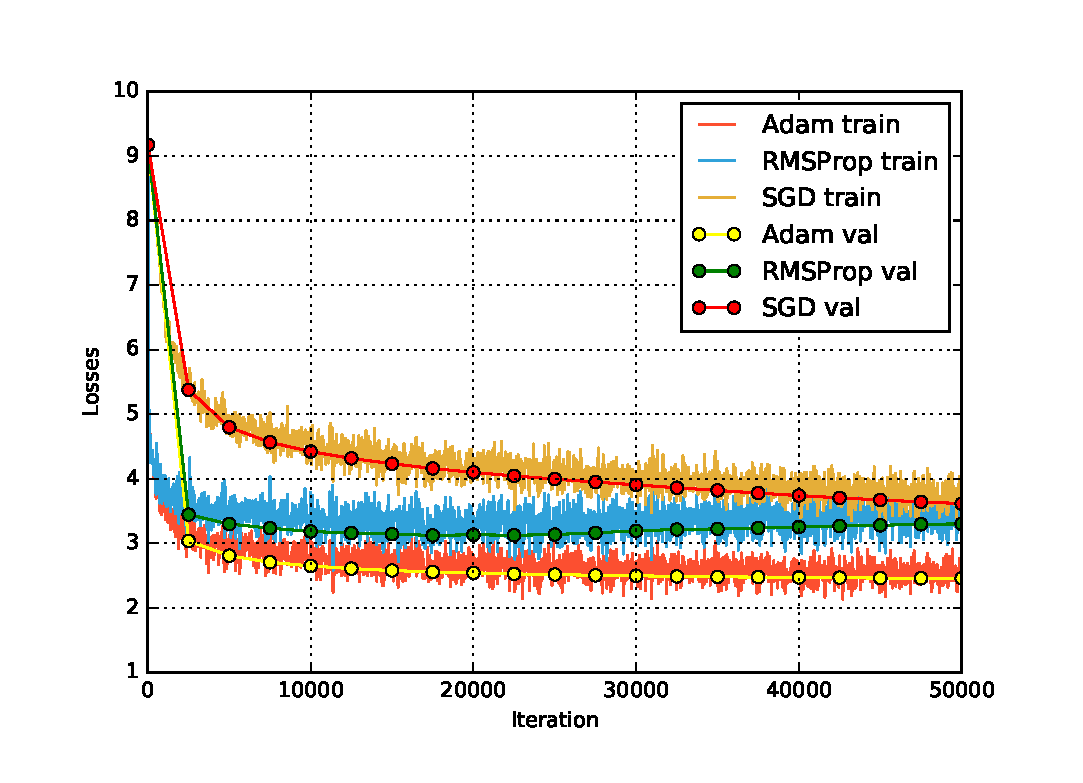
\includegraphics[width=0.48\linewidth]{Chapters/Fig/vgg_optims.eps}
			\hfill
			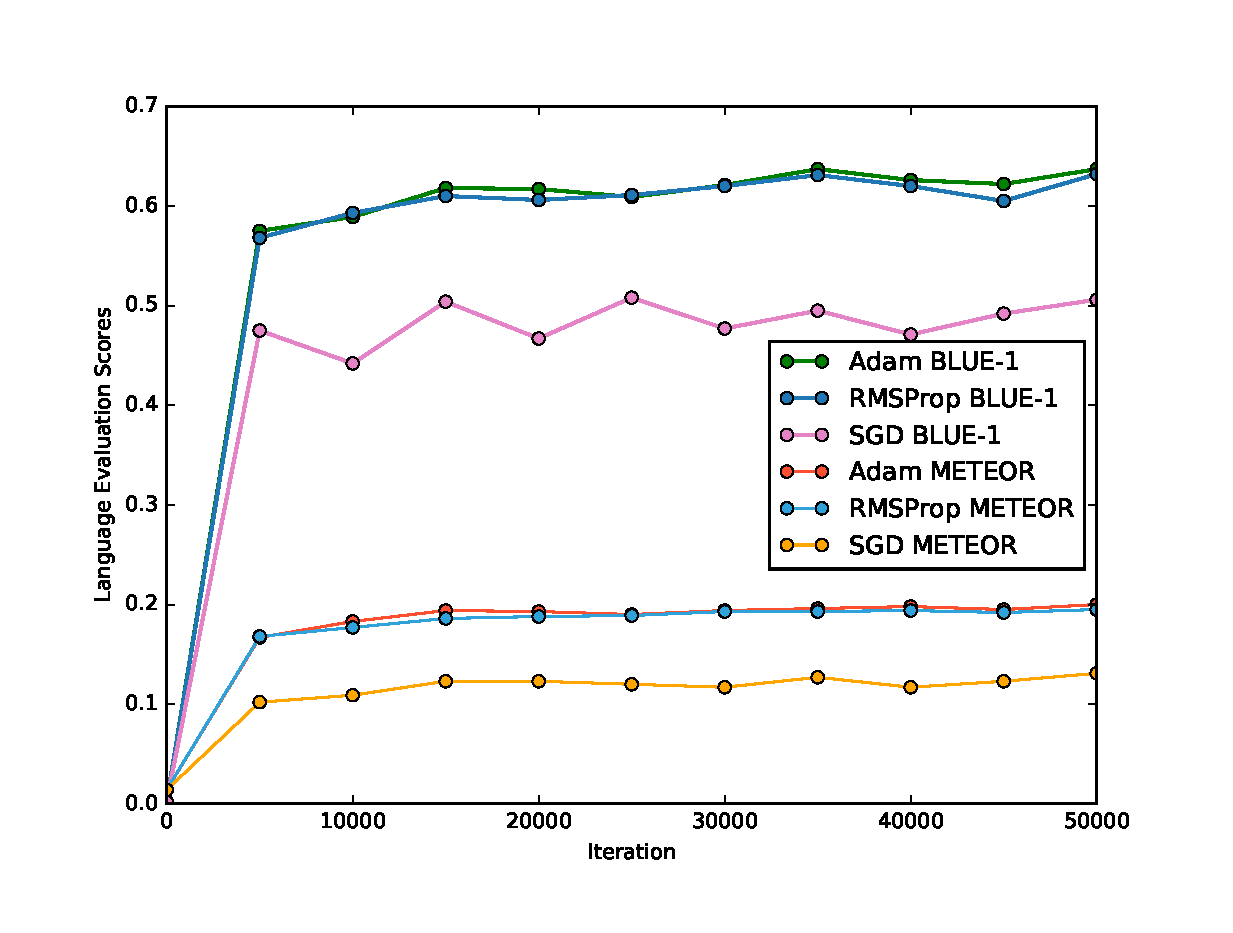
\includegraphics[width=0.48\linewidth]{Chapters/Fig/vgg_lang_stat.eps}
		}
		\subfigure[Config-2: AlexNet as CNN, LSTM with $512$ hidden units]{
			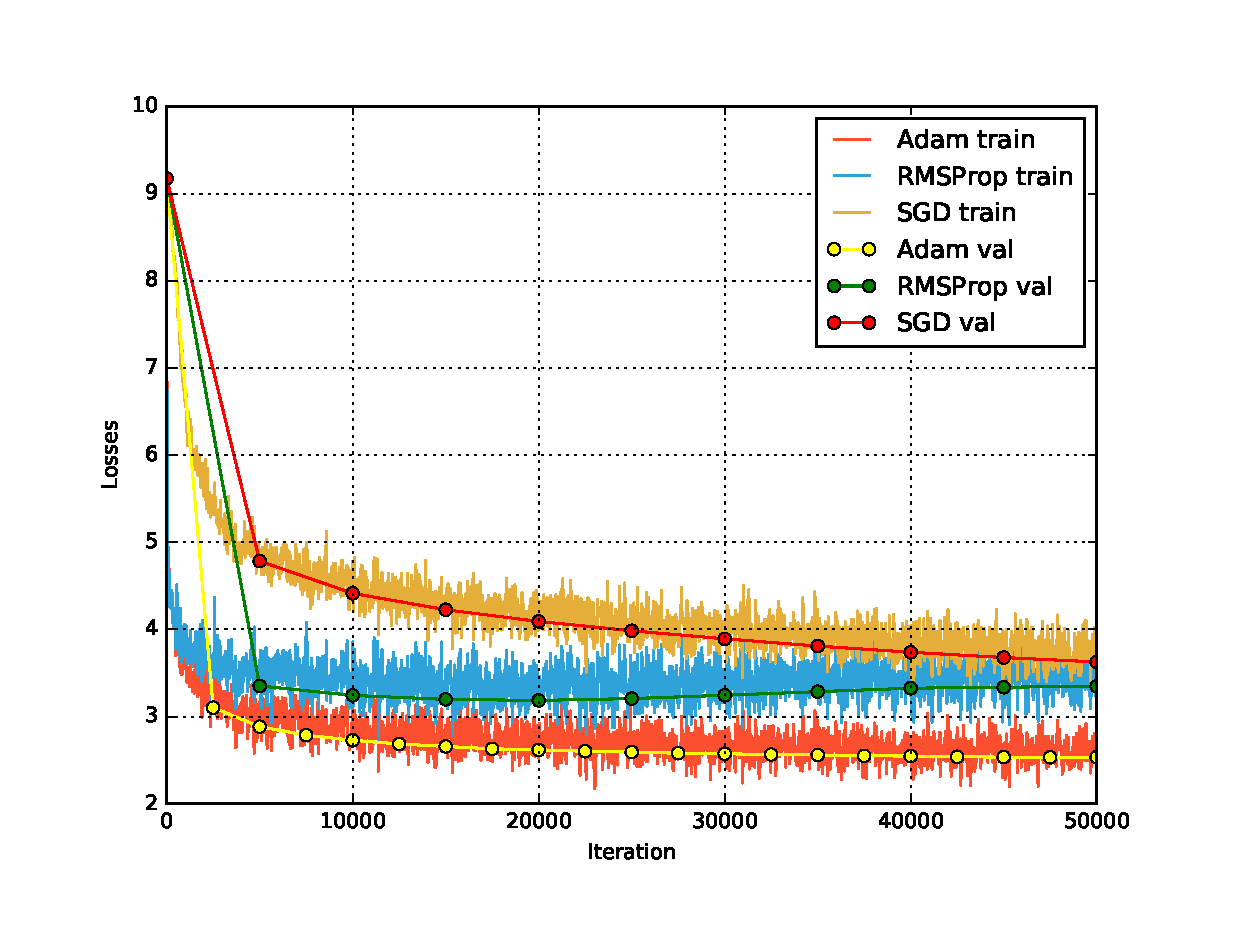
\includegraphics[width=0.48\linewidth]{Chapters/Fig/alex_optims.eps}
			\hfill
			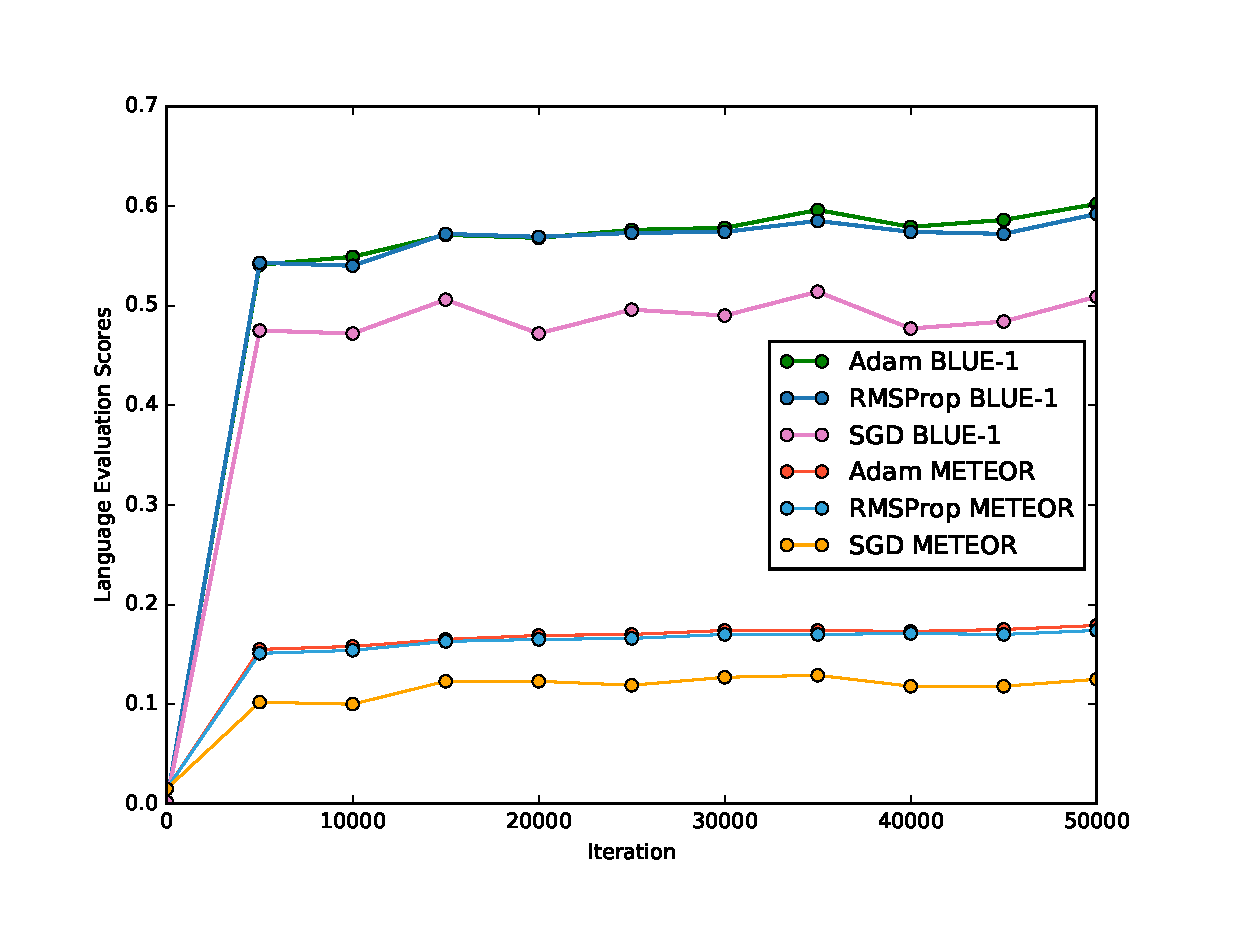
\includegraphics[width=0.48\linewidth]{Chapters/Fig/alex_lang_stat.eps}
		}
		\caption[Comparison of $3$ opitmization methods ]{Comparison of $3$ optimization methods: SGD, RMSProp and Adam w.r.t training/validation losses and language evaluation score during the first $50,000$ training iterations}
		\label{fig:exp1} % label should be placed immediately after \caption for cross-reference to work properly
	\end{figure}

The train and validation losses as well as language evaluation scores during the first $50,000$ iterations for each configuration are shown in \ref{fig:exp1}. 

As can be inferred from figure \ref{fig:exp1}, regardless of the \gls{cnn}, Adam optimizer gives the fastest convergence rate; pure \gls{sgd} without momentum and weight decay gives the lowest convergence rate compared the other optimization methods. In addition, the losses reach a ``plateau'' (approximately $2.5$) very quickly after about first $20,000$ iterations, which indicates that the chose learning rate is considerably good enough for this problem.  

Regarding the language evaluation scores on standard metrics, both Adam and RMSProp achieves superior results to SGD, with Adam performs slightly better. The BLEU-1 and METEOR scores for SGD is fluctuated, which reflects its lower convergence rate compared to Adam and RMSProp.

Following the monitoring stragies presented in section \ref{sec:monitoring}, I kept training and monitoring the behavoirs of the models with different settings. The training was terminated if the gradient is exploded (which did not happen for all experiments shown in this thesis) or when the CIDEr score was not improved after $50,000$ consecutive iterations to prevent overfitting. 

On hardware environment mentioned in section \ref{sec:hardware}:
\begin{itemize}
	\item Config-1
	\begin{itemize}
		\item \textit{Adam optimizer}: takes approximately $20$ hours to train and achieves the best results at iteration $94,000$-th. 
		\item \textit{RMSProp optimizer}: training time is $29,4$ hours and achieves the best results at iteration $138,000$-th.
		\item \textit{SGD optimizer}: training finished after $38,2$ hours and achieves the best results at iteration $272,000$-th
	\end{itemize}
	\item Config-2
	\begin{itemize}
		\item \textit{Adam optimizer}: takes approximately $23$ hours to train and achieves the best results at iteration $146,500$-th. 
		\item \textit{RMSProp optimizer}: training time is $30,3$ hours and achieves the best results at iteration $191,000$-th.
		\item \textit{SGD optimizer}: training finished after $42,5$ hours and achienves the best results at iteration $189,000$-th
	\end{itemize}
\end{hardware}

The BLEU, METEOR and CIDEr scores for this experiment are reported in Table \ref{tab:exp1_coco_score}

\renewcommand{\arraystretch}{1.2}

\begin{table}
	\centering
	\begin{tabular}{llcccccc}
		\toprule
		Configuration & Optimizer & B-1 & B-2 & B-3 & B-4 & METEOR & CIDEr \\ \midrule
		\multirow{3}{*}{\textit{Config-1}} & Adam & \textbf{62.9} & & & & 21.2 & \textbf{65.5} \\
		 & RMSProp & 61.8 & & & & 19.7 & 62.4 \\
		 & SGD & 55.5 & & & & 15.5 & 32.3 \\
		 \midrule
		 \multirow{3}{*}{\textit{Config-2}} & Adam & 61.5 & & & &\textbf{21.5} & 63.7 \\
		 & RMSProp & 60.2 & & & & 18.9 & 61.2 \\
		 & SGD & 53.1 & & & & 14.0 & 30.8 \\
		 \bottomrule
	\end{tabular}
	\caption{Scores on the MSCOCO development set}
	\label{tab:exp1_coco_score}
\end{table}

\textbf{Conclusion:} With both VGGNet and AlexNet as the CNN module of the model, Adam $\left( \eta = 5\mathrm{e}{-4}$; $\alpha = 0.8, \beta = 0.999, \epsilon = 1\mathrm{e}{-8} \right) $ gives the best results in terms of the model convergence rate. Hence, it will be used as the optimization method in the subsequent experiments.

\subsection{Experiment 2: LSTM Architecture}
\subsubsection{Experimental setup}
As studied in \cite{DBLP:journals/corr/GreffSKSS15}, beside the learning rate $\eta$, the hidden layer size $h$ is an important hyperparameter that affects the performance of \gls{lstm} network. 
This experiment is conducted to evaluate the effects of different hidden sizes $h$ to the captioning model so as to figure out a suitable one as a trade-off between the performance of the model and the required training time as well as the computational capability of machine used in inference phase.
To this end, I consider three different values of $h$ that are largely used in researches of \gls{lstm}. %, specifically $h = \left\{ 256, 512, 1000\right\}$. 
The learning rate is set to $\eta = 5\mathrm{e}{-4}$, and the optimization method is Adam.

\subsubsection{Experimental results and evaluations}
\begin{figure}[ht]
	\subfigure[VGGNet as CNN; Adam optimizer]{
		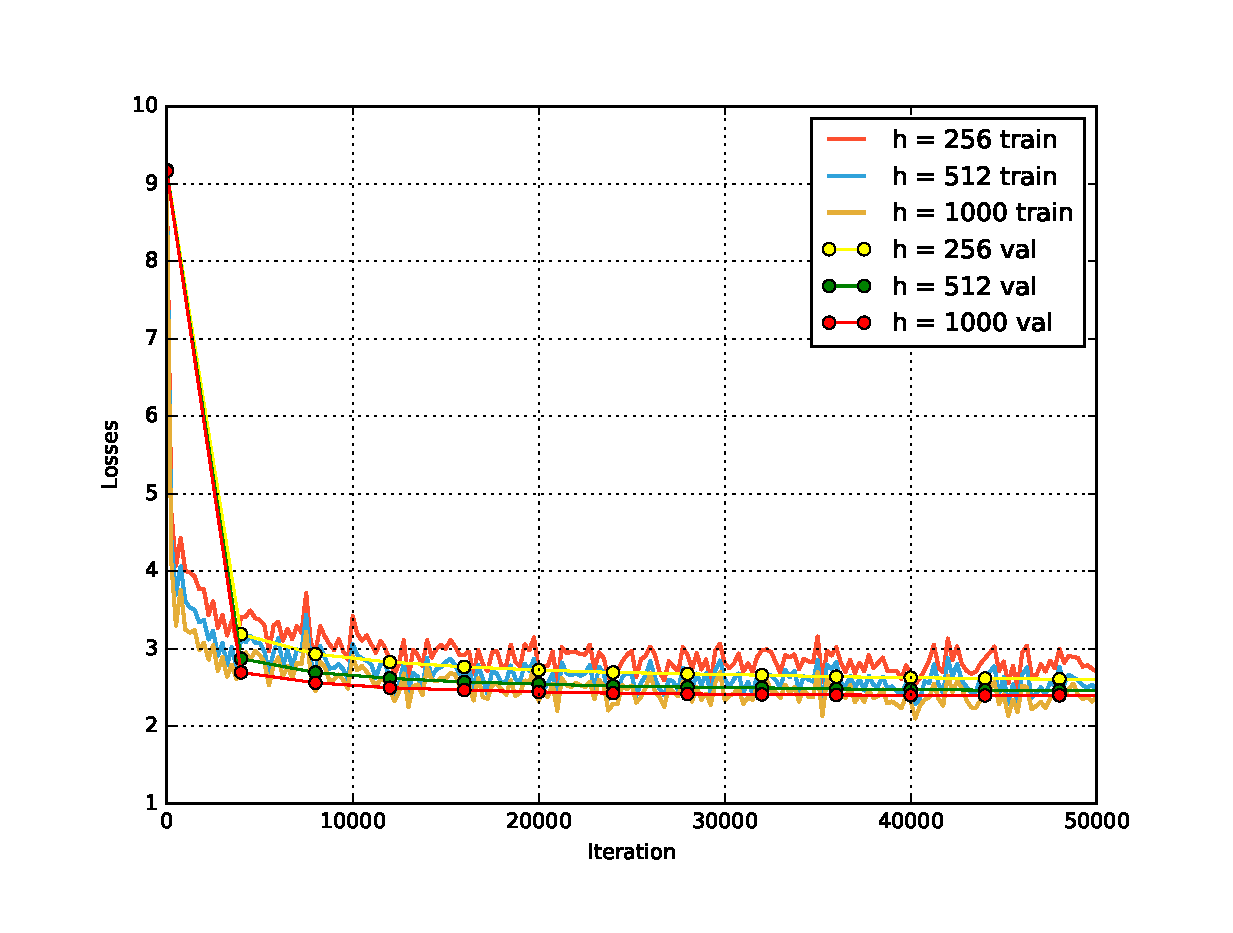
\includegraphics[width=0.48\linewidth]{Chapters/Fig/vgg_hiddens.eps}
		\hfill
		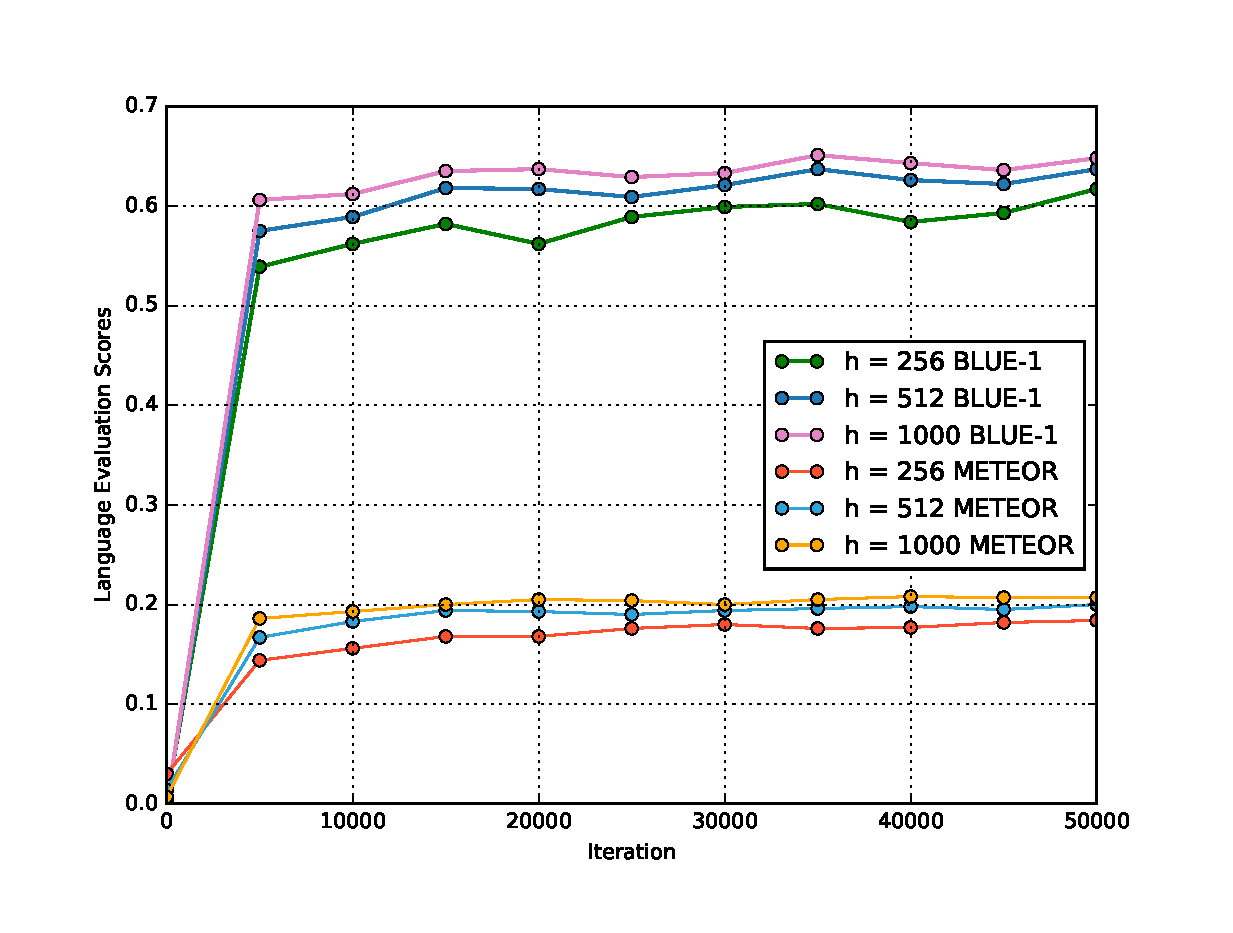
\includegraphics[width=0.48\linewidth]{Chapters/Fig/vgg_hidden_lang_stat.eps}
	}
	\subfigure[AlexNet as CNN; Adam optimizer]{
		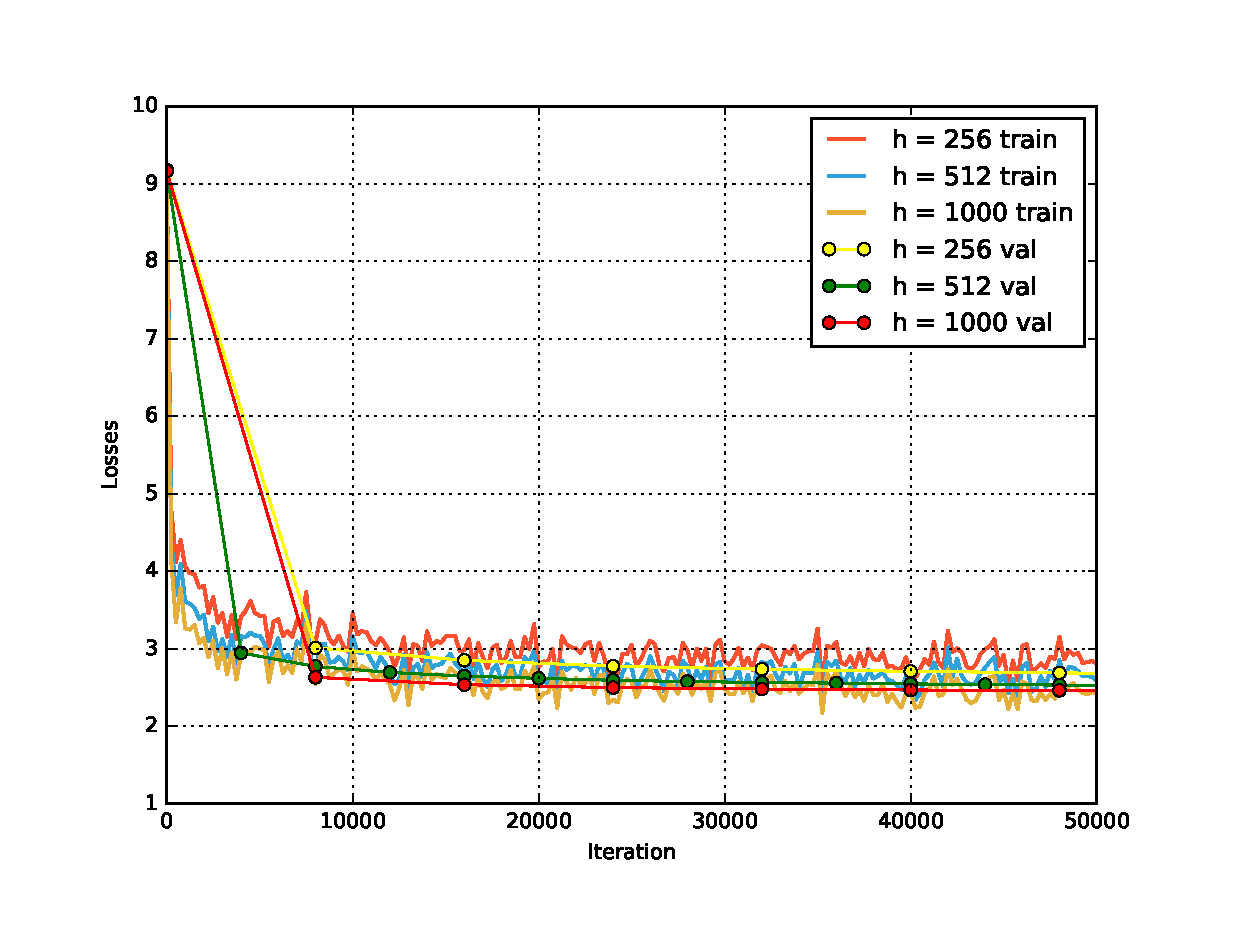
\includegraphics[width=0.48\linewidth]{Chapters/Fig/alex_hiddens.eps}
		\hfill
		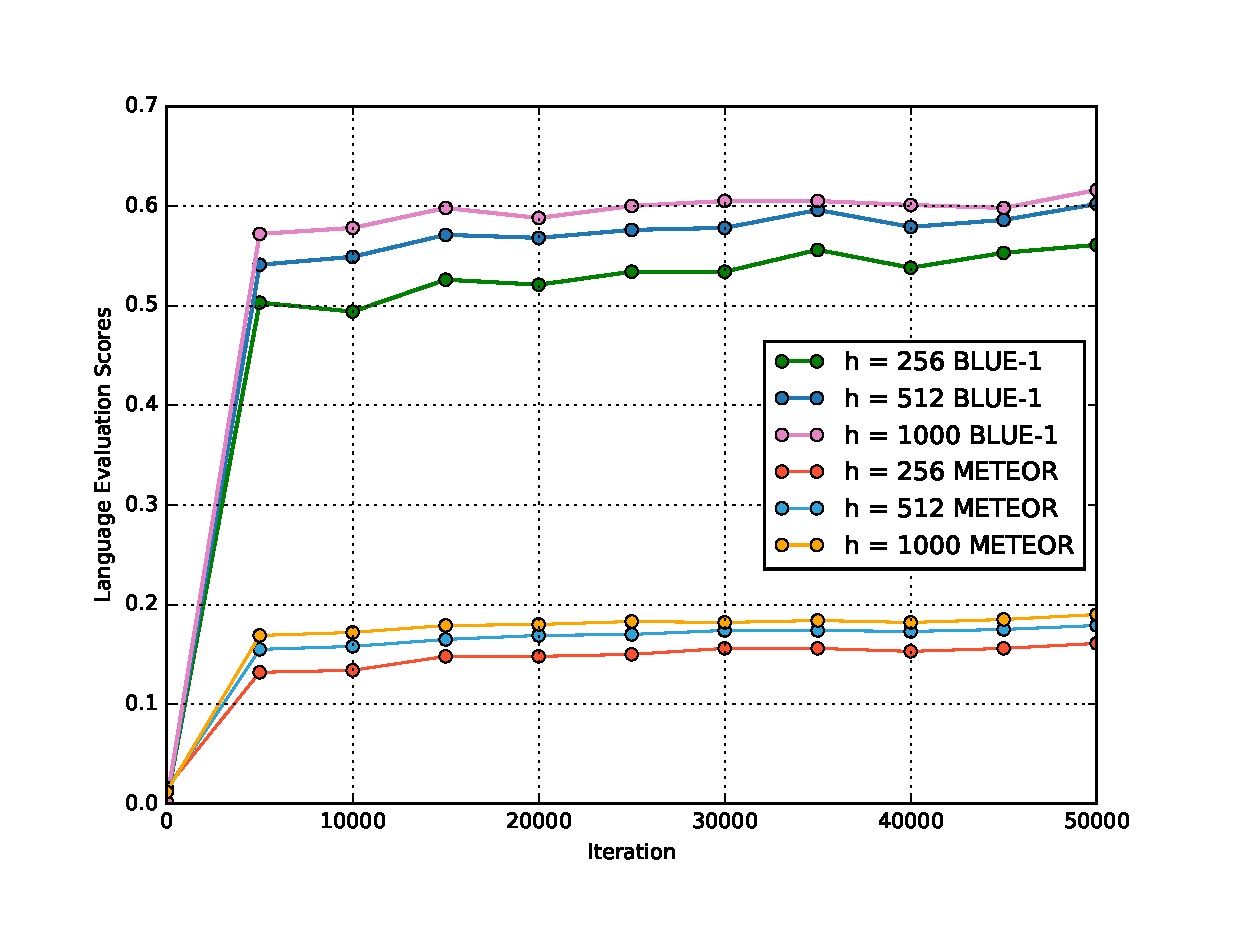
\includegraphics[width=0.48\linewidth]{Chapters/Fig/alex_hidden_lang_stat.eps}
	}
	\caption[Comparison of $3$ LSTM hidden sizes]{Comparison of $3$ LSTM hidden sizes: $h \in \left\{ 256, 512, 1000 \right\}$ w.r.t training/validation losses and language evaluation score during the first $50,000$ training iterations}
	\label{fig:exp2} % label should be placed immediately after \caption for cross-reference to work properly
\end{figure}

The plots in Figure \ref{fig:exp2} show that all three LSTM hidden sizes result in the remarkably similar convergence rates, both training and validation losses converges quickly. Furthermore, as expected, larger networks perform better,
however the required training time and the number of network's parameters are also considerably increased. As a result, the model might not be usable when it is deployed to different machines at the inference time even though inference is just forwarding the inputs to the model.

// \textit{TODO: Perform experiments on different LSTM architecture }
Another unexpected result of this experiment is that momentum affects neither performance nor training time in any significant way. ...
These observations suggest that momentum does not offer substaintial benefits when training LSTMs with online stochastic gradient descent as it does with the case of \gls{cnn}. It may, however, be more important in the case of batch training in which the gradient is less noisy.

\textbf{Conclusion:} In the context of this experiment, the differences of convergence rate and performance of the model are not significant amongst three hidden size values evaluated. Nonetheless, as predefined above, the ultimate goal of this experiment is not to point out the best model in some certain extents but to figure out the trade-offs between model's performance versus the feasibility of deploying that model to wide varieties of hardware infrastructure. To this end, the good choice is an LSTM with $h = 512$ and \texttt{tanh} nonlinearity for its forget gate.

\subsection{Experiment 3: AlexNet vs VGGNet}

\subsection{Experiment 4: Transfer learning}
